\section{Architecture}

WHAT follows an intransparent multitier architecture. 
The GUI, presentation logic, application processing, data accessing and storing data
are logically and also partly locally separated. Intransparent means that communication
between tiers just happens between adjacent ones. The different tiers are described below.


\begin{center}
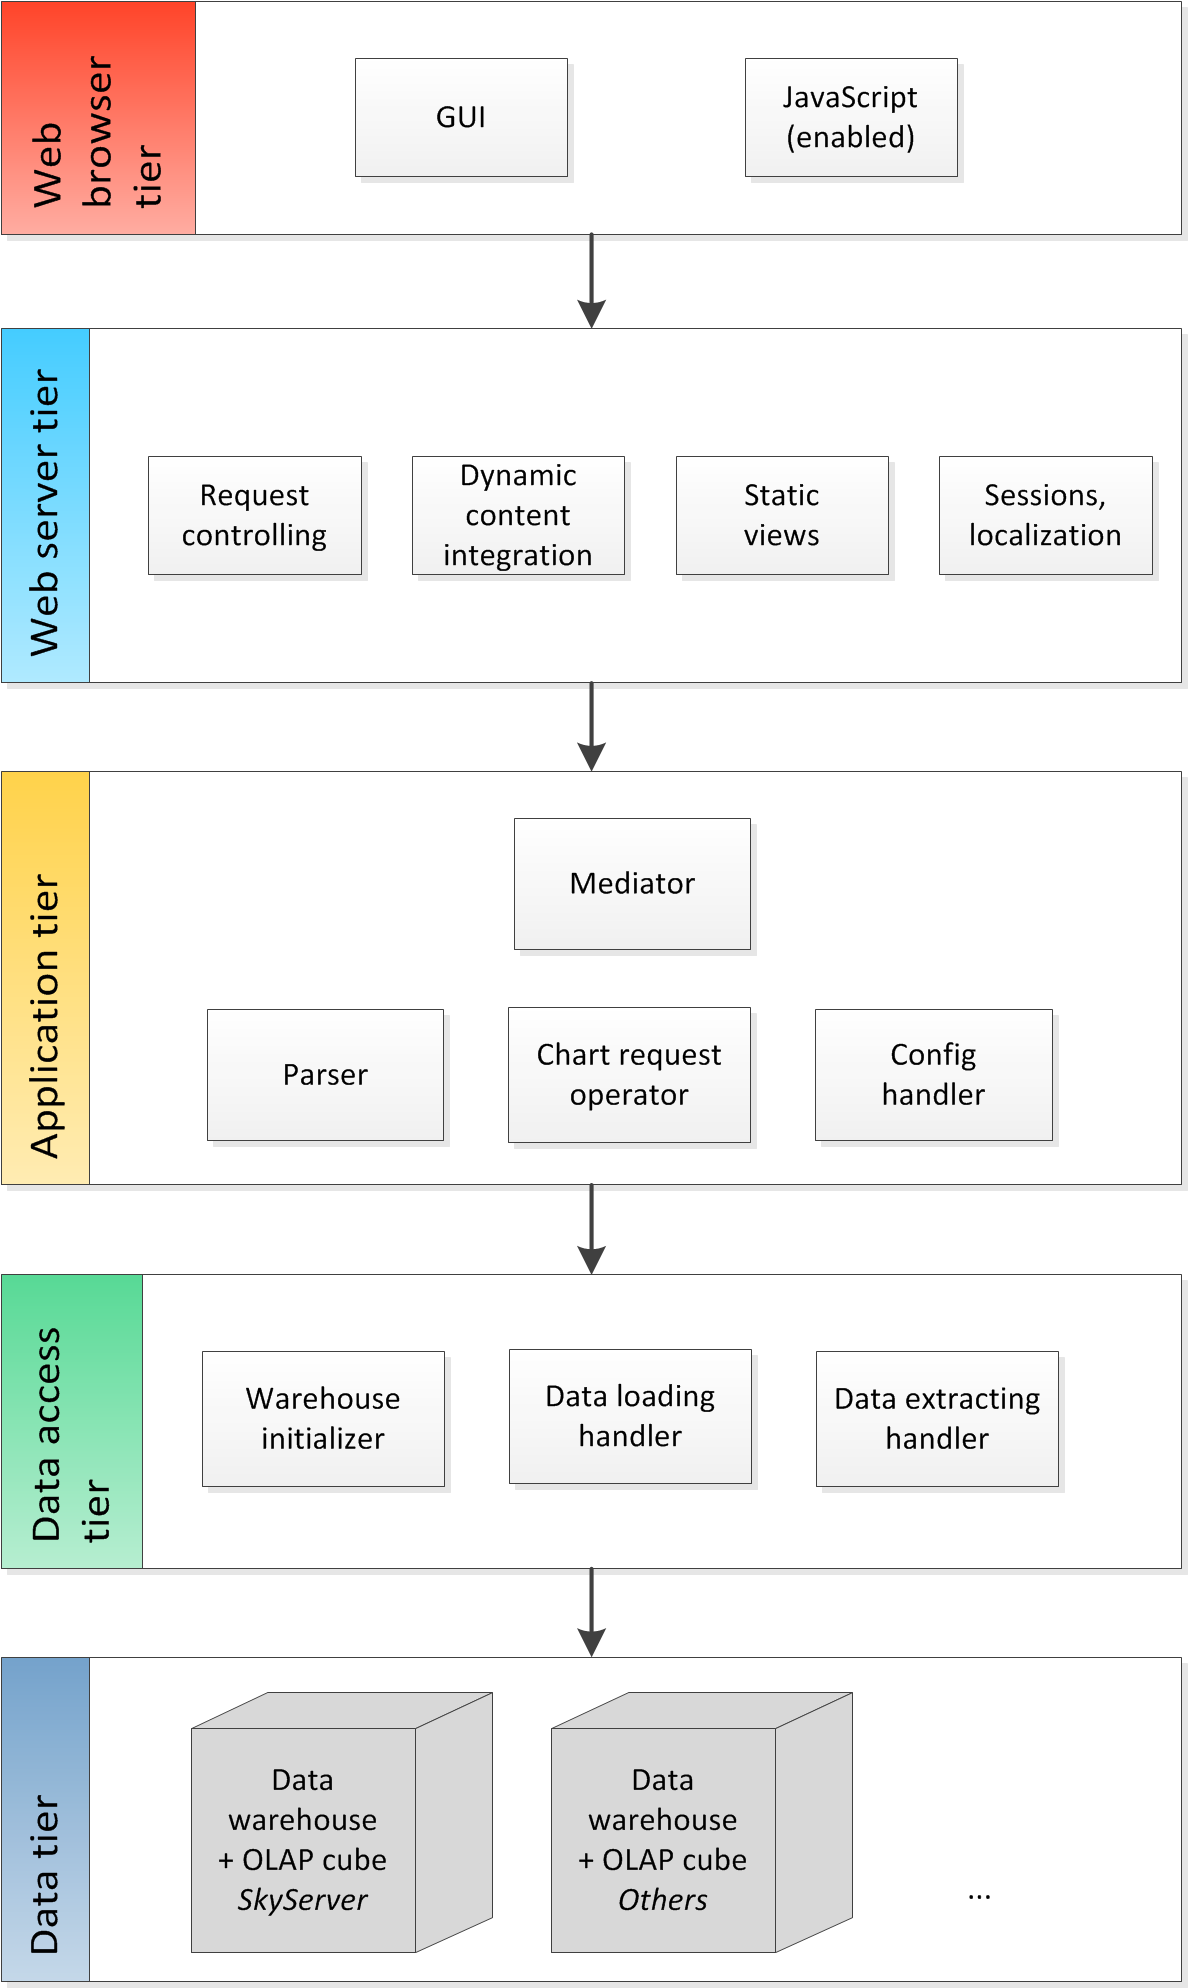
\includegraphics[width=0.6\linewidth]{Pictures/TierArchi.png} 
\end{center}   


\subsection{Web browser tier}
The web browser tier represents the GUI of the client, which will be displayed as web page.
In the following context GUI and web page will be used interchangeably, as they are they same thing.
The webpage utilizes javascript.
It handles part of the user interaction with the program.

%As the web page uses JavaScript, it has to be enabled in the browser. %Muessen wir die da reinscheiben?
%Besides this, Google Chrome and Firefox have to be supported. %


\subsection{Web server tier}
The web server provides the presentation logic. This includes both the serving of static files as well as
the dynamic integration of content in the html pages.
Other tasks are session handling, language localization and most importantly request handling.

It handles the rest of the user interaction with the webpage, while invoking the application tier when needed.
%Which means it handles the actions triggered on the web page and decides whether it can handle them itself 
%or pass them to application tier. Last one happens for example when a chart is requested. 
This tier uses and is tightly integrated with java Play Framework.


\subsection{Application tier}
The application tier's function is twofold.
On the one hand, it handles the parsing process and the management of configuration files.
On the other hand, it acts as a sort of middleman between the web server tier and the data access tier.
%Jo, ist ChartDataRequester teil vom Application tier oder vom Data access tier?

\subsection{Data access tier}
This tier manages all requests of loading and extracting data from the data tier. So its main task is
to build a bridge from the application in Java to the SQL language of the Oracle warehouses and OLAP-Cubes.
If there is enough time to implement this optional function, it will also handle 
the automatic initialization of new data warehouses.  

\subsection{Data tier}
In the data tier the data warehouses and their OLAP-Cubes are stored. 
This will be done with the Oracle software.  
